\documentclass[10pt,twoside]{article}
\usepackage[utf8]{inputenc}
\usepackage{amsmath}
\usepackage{amsfonts}
\usepackage{amssymb}
\usepackage[spanish,es-noshorthands]{babel}
\usepackage[T1]{fontenc}
\usepackage{lmodern}
\usepackage{graphicx,hyperref}
\usepackage{tikz,pgf}
\usepackage{multicol}
\usepackage{subfig}
\usepackage[papersize={6.5in,8.5in},width=5.5in,height=7in]{geometry}
\usepackage{fancyhdr}
\pagestyle{fancy}
\fancyhead[LE]{
\includegraphics[height=12pt]{Images/logo-colegio.png} Estadística $6^{\circ}$}
\fancyhead[RE]{}
\fancyhead[RO]{\textit{Germ\'an Avenda\~no Ram\'irez, Lic. U.D., M.Sc. U.N.}}
\fancyhead[LO]{}

\author{Germ\'an Avenda\~no Ram\'irez, Lic. U.D., M.Sc. U.N.}
\title{\begin{minipage}{.2\textwidth}

\includegraphics[height=1.75cm]{Images/logo-colegio.png}\end{minipage}
\begin{minipage}{.55\textwidth}
\begin{center}
Taller 03, Tablas de Frecuencia  \\
Estadística $6^{\circ}$
\end{center}
\end{minipage}\hfill
\begin{minipage}{.2\textwidth}

\includegraphics[height=1.75cm]{Images/logo-sed.png} 
\end{minipage}}
\date{}
\begin{document}
\maketitle
Nombre: \hrulefill Curso: \underline{\hspace*{44pt}} Fecha: \underline{\hspace*{2.5cm}}
\section*{Aprendo algo nuevo}
Observe cómo registraron la información sobre el peso de un grupo de estudiantes Milena y Simón.
\begin{center}
\begin{tabular}{|c|p{3.5cm}|p{6cm}|}
\hline 
Peso en kg & Número de alumnos (Frecuencia) & Parte del total de alumnos que tienen ese peso \\ 
\hline 
41 & 1 & 1/10 \\ 
\hline 
43 & 1 & 1/10 \\ 
\hline 
47 & 2 & 2/10 \\ 
\hline 
49 & 4 & 4/10 \\ 
\hline 
52 & 2 & 2/10 \\ 
\hline \hline
Total & 10 & 10/10=1 \\ \hline
\end{tabular} 
\end{center}
\subsection*{Actividad 1}
\begin{itemize}
\item ¿Cuántos datos se registraron en esa actividad?
\item ¿Cuántas estudiantes del total pesan 41 kilogramos?
\item ¿Cuántos pesan 49?
\end{itemize}
La tercera fila de esa tabla, da información sobre qué parte de la población en estudio o de una de muestra (parte de la población), corresponde a la característica analizada. Esos valores se conocen como frecuencias relativas.

Por ejemplo, la frecuencia relativa que corresponde a 47 kilogramos es 2/10, es decir de diez estudiantes dos pesan 47 kilogramos.
\begin{itemize}
\item ¿Cuál es la frecuencia absoluta de 49 kilogramos?
\item ¿Cuál es la frecuencia relativa del mismo peso? ¿Qué significa ese valor?
\end{itemize}
Milena y Simón siguen completando datos en la tabla.
Analiza y en tu cuaderno, completa la tabla.
\begin{center}
\begin{tabular}{|c|c|c|c|c|}
\hline 
Peso en & Número de & Parte del total & Frecuencia & Frecuencia \\ 
kg & alumnos & de alumnos que & acumulada & acumulada \\ 
 & (Frecuencia) & tienen ese peso & absoluta & relativa \\ 
\hline 
41 & 1 & 1/10 & 1 & 1/10 \\ 
\hline 
43 & 1 & 1/10 & 2 & 2/10 \\ 
\hline 
47 & 2 & 2/10 & 4 &  \\ 
\hline 
49 & 4 & 4/10 &  &  \\ 
\hline 
52 & 2 & 2/10 & & \\ \hline \hline
Total & 10 & 10/10=1 & & \\ \hline
\end{tabular} 
\end{center}
\begin{itemize}
\item ¿Cuántos estudiantes de la clase de Milena, pesan 49 kilogramos o menos?
\item ¿Qué parte de esos estudiantes pesan 49 kilogramos o menos?
\end{itemize}
Consigue una calculadora, y halla el cociente de dividir la cantidad de estudiantes que pesan 49 kilogramos o menos entre 10.

El cociente que se obtiene, 0.8, quiere decir que aproximadamente el 80\% de los compañeros de Milena y Simón pesan 49 kilogramos.

Completa la tabla en tu cuaderno escribiendo el porcentaje de cada dato.\\

 \fbox{\begin{minipage}{.95\textwidth}\emph{Para cierto valor de una característica de una población o una muestra, la frecuencia acumulada relativa se calcula mediante el cociente de la frecuencia acumulada del dato y el número total de datos.}\end{minipage}}
\section*{Ejercito lo aprendido}
\subsection*{Actividad 2}
\begin{enumerate}
\item Santiago recogi\'{o} la siguiente informaci\'{o}n acerca de las estaturas de sus compañeros.
\begin{center}
\begin{tabbing}
\hspace{1.5cm}\=\hspace{1.5cm}\=\hspace{1.5cm}\=\hspace{1.5cm}\=\kill
 142 \> 143 \> 146 \> 142 \> 145\\ 
140 \> 138 \> 143 \> 146 \> 142 \\ 
139 \> 139 \> 142 \> 143 \> 142\\ 
145 \> 137 \> 147 \> 143 \> 143
\end{tabbing} 
\end{center}
Construyan una tabla en donde aparezcan las frecuencias absolutas y relativas correspondientes a los datos de la estatura en centímetros de los 20 estudiantes de la escuela.

Respondan:
\begin{enumerate}
\item ¿Cuál es la mayor frecuencia absoluta?
\item ¿A qué dato corresponde?
\item ¿Cuál es la menor frecuencia absoluta?
\item ¿A qué dato corresponde?
\item ¿Cuántos compañeros de Santiago miden 142 cm?
\item ¿Qué porcentaje de estudiantes tiene una estatura de 138 cm?
\end{enumerate}
\section*{Evaluaci\'{o}n}
\item A 15 estudiantes de postprmaria se les preguntó por el número de hermanos que cada uno tiene. Las respuestas se presentan a continuación.
\begin{center}
2, 2, 3, 1, 1, 0, 0, 0, 3, 2, 2, 2, 4, 2, 2
\end{center}
\begin{enumerate}
\item Ordenen los datos de menor a mayor.
\item Construyan una tabla de frecuencias absolutas y relativas para el número de hermanos.
\item ¿Cuántos estudiantes son hijos únicos?
\item ¿Cuántos no lo son?
\item ¿Cuántos alumnos tienen el mayor número de hermanos? 
\item ¿Cuál es el número de hermanos que tiene la mayoría de los estudiantes?
\item ¿Qué porcentaje de estudiantes encuestados tienen tres hermanos?
\item ¿Qué porcentaje tiene solo un hermano?
\end{enumerate}
\end{enumerate}
\section*{Otra forma de ver los datos recogidos}
Observe el siguiente diagrama
\begin{center}
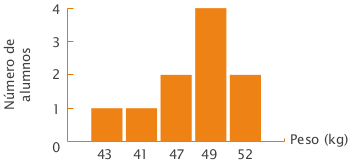
\includegraphics[scale=.75]{Images/diagrama_barras.png} 
\end{center}
\subsection*{Actividad 3}
\begin{itemize}
\item ¿Qué información está representada en él?
\item ¿Sabes que nombre recibe esa representación?
\item ¿Cómo sabes cuál es el dato con mayor frecuencia?
\item ¿Y el dato con la menor frecuencia?
\item ¿Cuántos estudiantes pesan 52 kilogramos?
\item ¿Qué dato tiene una frecuencia de 2?
\item Explica de qué manera lees la información que está representada.
\end{itemize}
\subsection*{Aprendo algo nuevo}
\fbox{\begin{minipage}{.95\textwidth}
\emph{Las diferentes características de una población pueden representarse de varias maneras. Entre ellas se encuentran: las tablas de frecuencia, los diagramas de barras o los diagramas circulares.}
\end{minipage}}
La representación anterior corresponde a un diagrama de barras. Observe nuevamente el diagrama anterior.

\end{document}
